\documentclass[10pt]{article}
\usepackage[margin=0.9in]{geometry}
\usepackage[T1]{fontenc}
\usepackage{lmodern}
\usepackage{amsmath,amssymb,booktabs,graphicx,array}
\usepackage[colorlinks=true,allcolors=blue]{hyperref}
\usepackage{microtype}
\setlength{\parskip}{0.35em}
\setlength{\parindent}{0pt}
\renewcommand{\topfraction}{0.95}
\renewcommand{\bottomfraction}{0.95}
\renewcommand{\textfraction}{0.05}
\renewcommand{\floatpagefraction}{0.85}
\clubpenalty=10000
\widowpenalty=10000
\newcommand{\ent}{\textsc{Entailment}}
\newcommand{\con}{\textsc{Contradiction}}
\title{Sensitivity to Written Reasoning and Activation Steering:\\
Interim Results from a Controlled NLI Study\\[0.5em]
\large Working draft --- primary checkpoint comparison incomplete}
\author{Author details pending}
\date{2 November 2026}
\begin{document}
\maketitle
\begin{abstract}
We report a completed experiment on DeepSeek-R1-Distill-Qwen-7B using 50
held-out premise pairs, activation steering with equal-norm controls, and direct
changes to generated reasoning. Replacing a reasoning prefix with the trace
generated for the paired contradiction hypothesis changes 33 of 34 initially
correct eligible answers to contradiction; regenerating the answer from the
original full prefix changes none of those 34. Shortening the original prefix
does not produce a clear accuracy decline in this small sample. Across 64 paired
activation-versus-control comparisons, the smallest unadjusted exact $p$-value
is 0.0625, and none is significant after Holm adjustment. A review also identifies
an incorrect automated reasoning verdict, so disagreement labels require further
validation. These results establish sensitivity to the inserted text under the
tested interventions; they do not identify mediation through naturally generated
reasoning. The Distill-32B experiment remains incomplete and QwQ-32B results are
not available in this report. The planned comparison of the two 32B checkpoints
therefore remains pending.
\end{abstract}

\section{Scope and evidence status}
The study asks how changes to hidden activations and written reasoning affect
final answers on a binary natural-language inference task. Its primary planned
comparison is DeepSeek-R1-Distill-Qwen-32B versus QwQ-32B. This interim report
concerns the completed 7B study, which contains 5,229 generation records, and a
timestamped baseline snapshot from the ongoing Distill-32B study. The experiment
uses inference-time interventions within checkpoints; it does not randomly assign
models to training methods. No difference observed between checkpoints should be
attributed solely to supervised fine-tuning, reinforcement learning, or scale.

Generation settings were frozen locally after calibration. This is a recorded
local protocol, not an external preregistration. The supplementary analysis was
specified locally before held-out outcome tables were available, but its tests
and intervals are exploratory. This document is a separate working report;
it neither replaces the primary manuscript nor presents the campaign as complete.

\section{Methods}
\subsection{Data, model, and generation}
Each SNLI contrast pair shares a premise and contains one entailment hypothesis
and one contradiction hypothesis. The construction, calibration, and evaluation
partitions contain 500, 50, and 50 pairs, respectively, from the official training,
validation, and test splits. Normalized premises are disjoint across partitions.
The resulting task excludes neutral labels and is not the conventional
three-class SNLI evaluation.

The completed experiment uses DeepSeek-R1-Distill-Qwen-7B with NF4 quantization
and a pinned model revision. Native chat templates request an explicit final
label. Sampling uses temperature 0.6, top-$p$ 0.95, top-$k$ 20, seed 42, and
batches of 16. Initial generations allow at most 2,048 new tokens. Both hypotheses
have their own unsteered baseline. Full prompts, token IDs, generated text,
sampling seeds, parse status, and stopping reason are retained. Invalid labels
and unfinished thought blocks are not silently converted into valid outcomes.

\subsection{Activation and text interventions}
At layer $l$, a direction $d_l$ is the difference between mean final-prompt-position
activations for contradiction and entailment prompts, estimated from the 500
construction pairs. We add $\alpha d_l$ for the first 15 prediction positions,
including the final prefill position. Eight zero-based layers
$\{0,4,8,12,16,20,24,27\}$ and four intensities
$\alpha\in\{0.5,1,2,4\}$ yield 32 steering conditions. Each condition has two
equal-norm controls: a random Gaussian direction, and a random direction
orthogonal to $d_l$. Control directions are seeded by example and layer and remain
fixed over the intervention positions. All 96 activation conditions use the same
50 entailment examples. Each condition has one seeded generation per example;
the study does not estimate variability across generation seeds.

For the 48 examples with a completed, parseable entailment baseline, text
interventions retain 0\%, 25\%, 50\%, 75\%, or 100\% of the reasoning tokens,
close the thought block, and regenerate up to 128 answer tokens. The full-prefix
condition controls for answer regeneration. Other conditions shuffle the original
reasoning tokens or substitute the trace generated for the paired contradiction
hypothesis. Substitution requires both traces to be available, leaving 41
examples, of which 34 had a correct initial entailment answer. A 0\% prefix
removes the original written reasoning; it does not remove the prompt, internal
computation, or the opportunity to generate further text.

\subsection{Outcomes, pairing, and missingness}
Accuracy counts absent or invalid final labels as incorrect. Contradiction rates
and treatment-minus-control differences are paired by example. Conditional flip
analyses use examples whose initial entailment answer was correct, with explicit
counts for missing intervention labels. If $f$ flips and $m$ missing labels occur
among $n$ eligible examples, the sample's missing-outcome bounds are
$[f/n,(f+m)/n]$; these are not sampling confidence intervals.

We use two-sided exact tests conditional on the number of discordant pairs
(the exact McNemar test). Holm adjustment covers the 64 activation/control
comparisons within the 7B model. Text contrasts are reported without adjustment
and remain exploratory. Paired bootstrap intervals resample examples using
5,000 draws; balanced baseline accuracy resamples the two hypotheses together
as a premise cluster. Repeated conditions on the same premise are not additional
independent observations. Complete-case comparisons can be biased if missingness
depends on the intervention.

\section{Results from the completed 7B experiment}
\subsection{Baseline competence}
The model answers 40/50 entailment examples and 42/50 contradiction examples
correctly. Respectively, 48 and 43 final labels are parseable; the remaining
2 and 7 traces reach the length limit without completing the thought block.
Balanced accuracy is 82\%, with a premise-cluster bootstrap 95\% interval
of 75--89\%. There are only 50 independent evaluation premises.

\subsection{Substitution strongly changes answers}
Among the 34 initially correct substitution-eligible examples, the contradiction
trace changes 33 answers to \con{} (97.1\%; Wilson 95\% interval 85.1--99.5\%).
The full original prefix yields no contradiction answers in these same 34
examples. All outcomes in this paired comparison are parseable. Its 33 discordant
pairs all favor increased contradiction, giving an unadjusted exact
$p=2.33\times10^{-10}$.

Across all 41 substitution-eligible examples, including initial errors,
contradiction answers rise from 7 under the full original prefix to 40 after
substitution. The paired difference is 80.5 percentage points (exploratory
bootstrap 95\% interval 68.3--92.7). This is the same set of 33 discordant pairs,
not an independent replication of the conditional result. Neither result uses
the automated reasoning assessor.

The inserted trace comes from a different hypothesis and may explicitly state
that hypothesis and its conclusion. Consequently, the observed effect does not
distinguish following intermediate reasoning from copying a conclusion or
accepting incompatible context. It demonstrates answer sensitivity to this
replacement, not causal mediation through naturally generated reasoning.

\subsection{Shorter prefixes show no clear accuracy decline}
Table~\ref{tab:truncation} uses the same 48 examples for all truncation levels.
The full prefix reproduces all 48 original parseable labels, including the eight
initial errors. Accuracy varies between 40/48 and 43/48 as the prefix is
shortened. These observations neither establish equivalence nor show that
shortening improves performance. At 0\%, two final labels are missing; the
complete-case contradiction comparison with 100\% has 46 pairs, with three
changes toward contradiction and five in the reverse direction ($p=0.727$).

\begin{table}[htbp]
\centering
\caption{Accuracy after retaining a fraction of the original reasoning prefix.
The denominator is the same 48 eligible examples, including initial errors.
Missing final labels count as incorrect. Intervals are Wilson 95\% intervals
for each accuracy, not intervals for paired differences.}
\label{tab:truncation}
\begin{tabular}{rrrrr}
\toprule
Retained & Correct & Accuracy & 95\% interval & Missing labels\\
\midrule
100\% & 40/48 & 83.3\% & 70.4--91.3\% & 0\\
75\%  & 40/48 & 83.3\% & 70.4--91.3\% & 0\\
50\%  & 41/48 & 85.4\% & 72.8--92.8\% & 0\\
25\%  & 43/48 & 89.6\% & 77.8--95.5\% & 0\\
0\%   & 41/48 & 85.4\% & 72.8--92.8\% & 2\\
\bottomrule
\end{tabular}
\end{table}

Shuffling the original tokens changes 8 of the 40 initially correct answers to
contradiction, versus none with the full prefix (unadjusted $p=0.0078125$).
However, this subset excludes possible corrections of initial errors. Across
all eligible examples with both labels observed, shuffling produces eight
changes toward contradiction and four away from it ($n=47$, $p=0.388$).
One shuffled answer is missing. Both views are needed to characterize this
intervention; the conditional flip rate is not an overall accuracy effect.
Figure~\ref{fig:text} summarizes the paired text contrasts and missingness bounds.

\subsection{No compelling activation effect relative to controls}
None of the 64 steering/control comparisons is significant after within-model
Holm adjustment; all adjusted $p$-values are 1. The smallest unadjusted exact
$p$ is 0.0625, for layer 0 at intensity 2 versus the Gaussian control. That
comparison has 38 complete pairs among 40 initially correct eligible examples,
with five discordant pairs favoring steering and none favoring the control.
Its complete-case difference is 13.2 percentage points. This selected extreme
is not confirmatory evidence. The small sample and missing outcomes also mean
that lack of significance should not be interpreted as proof of no effect.
Figure~\ref{fig:activation} displays all paired activation/control differences.

\begin{figure}[!htbp]
\centering
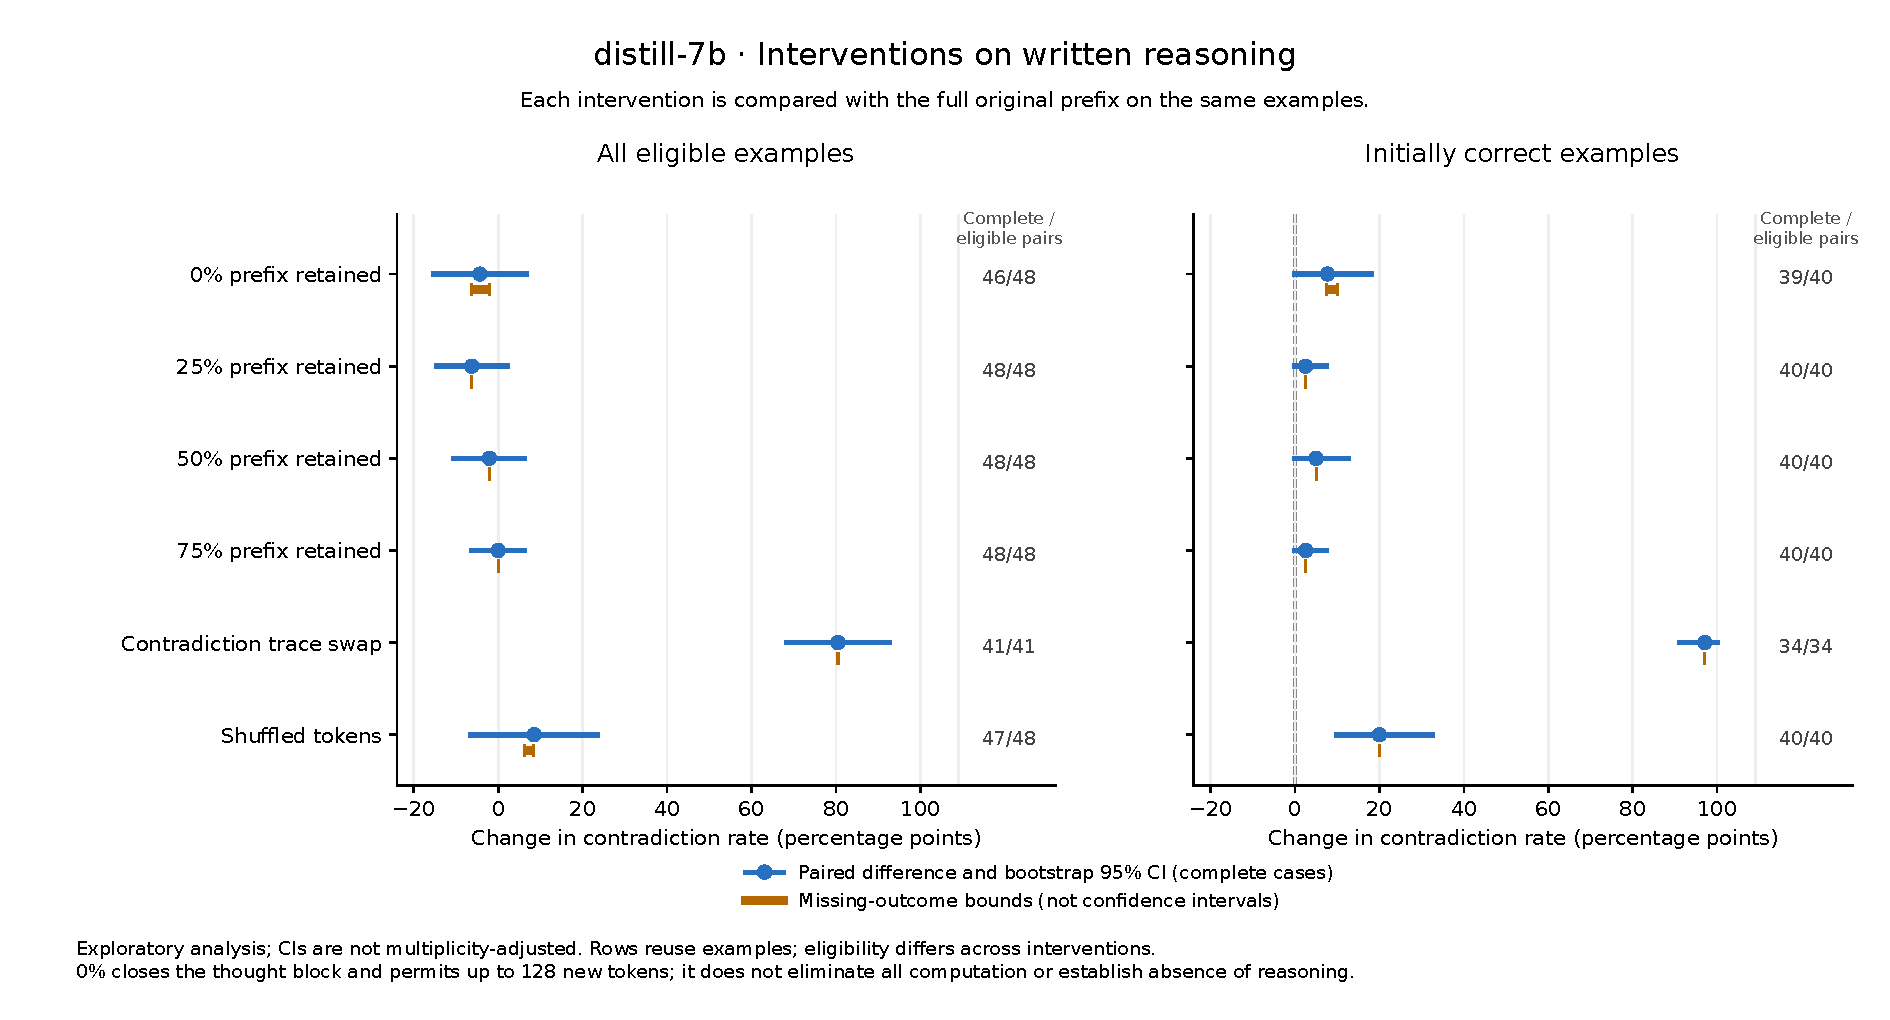
\includegraphics[width=\textwidth,height=0.60\textheight,keepaspectratio]
{../artifacts/diagnostics/20261102/figures/text_paired_contrasts.pdf}
\caption{Text interventions compared with answer regeneration from the full
original reasoning prefix. All-eligible and initially correct subsets are shown
separately. Points and bootstrap intervals describe paired complete-case
contradiction-rate differences; missingness bounds describe uncertainty from
unobserved labels in the observed sample, not sampling uncertainty. The same
examples contribute to multiple rows, and the two subsets overlap.}
\label{fig:text}
\end{figure}

\begin{figure}[!htbp]
\centering
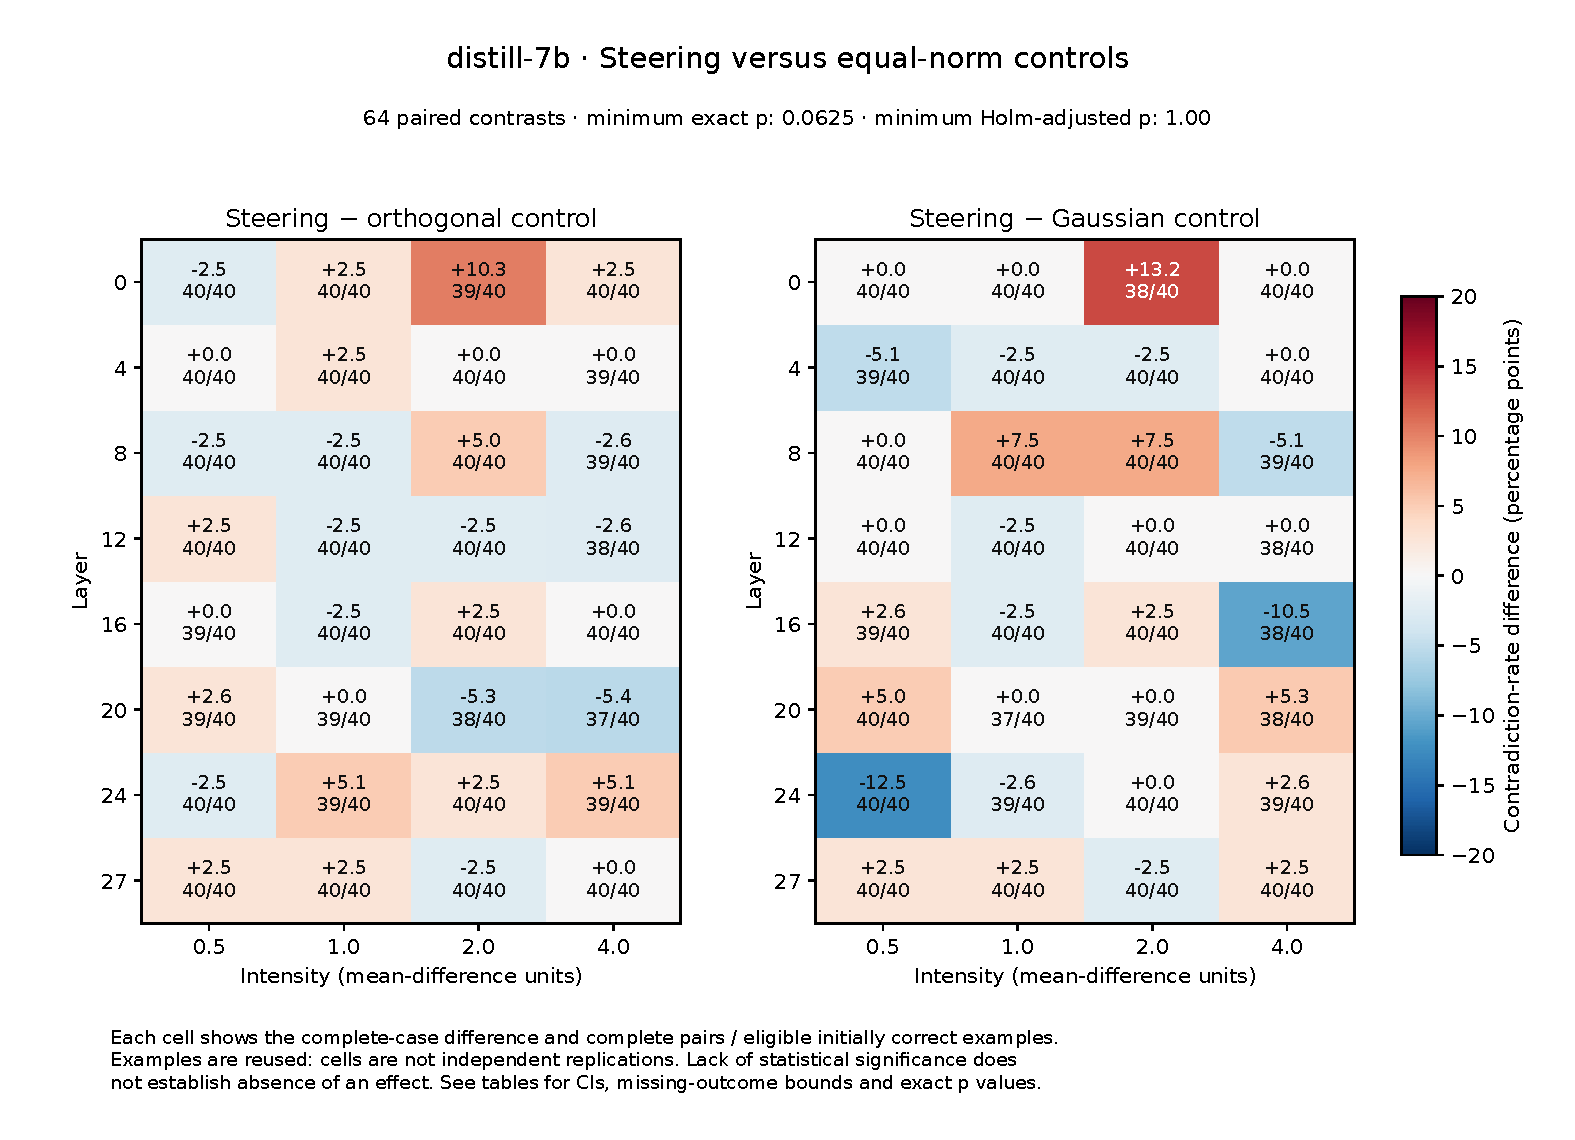
\includegraphics[width=\textwidth,height=0.55\textheight,keepaspectratio]
{../artifacts/diagnostics/20261102/figures/activation_control_contrasts.pdf}
\caption{Paired differences in contradiction rates between semantic steering
and equal-norm controls among initially correct 7B examples with both labels
observed. Cells repeat the same evaluation examples. None of the 64 exact
comparisons is significant after Holm adjustment; the heatmap is descriptive
and should not be read as identifying a privileged layer or intensity.}
\label{fig:activation}
\end{figure}

\section{Automated reasoning judgments require validation}
The assessor sees the reasoning text without the final answer and returns a
verdict with exact supporting quotations. The completed assessment file covers
4,850 baseline/activation records: 4,666 assessments are marked successful,
124 generations are incomplete, and 60 assessments return errors. The resulting
categories include 28 forward reasoning--answer mismatches and 14 reverse
mismatches. These are automated labels across repeated conditions, not 42
independently verified inconsistencies.

A concrete failure appears in the layer-0, intensity-2 steering record for
example \texttt{2ebc92fd4bda7938}. The generated reasoning ends:
\begin{quote}
``The hypothesis is the opposite of what's stated in the premise, so they
contradict each other.''
\end{quote}
The final answer is \con{}. The assessor quotes that sentence and describes
its conclusion as contradiction, yet returns an \ent{} verdict. The derived
mismatch category is therefore incorrect in this case. The reasoning may itself
misread the task, but task correctness and agreement with the reasoning's stated
conclusion are different measurements.

Schema checks and exact quotation matching did not detect this semantic error.
Likewise, the recorded retest agreement of 1.0 on 49 successful paired retests
does not establish validity. The original judgments must remain preserved.
Independent human review of flagged cases and a sample of unflagged cases is
needed before disagreement rates support substantive claims.

An exploratory assistant review read all 42 flagged records, representing eight
unique examples and 23 distinct reasoning texts. It proposed the transitions in
Table~\ref{tab:audit}. Under this reading, none remained a clear case of opposite
binary conclusions. This is an audit finding, not a validated correction or a
claim that the model has no reasoning--answer disagreements. The reviewer could
see the original labels, three flagged cases received only medium confidence,
and there was no independent human adjudication. A seeded sample of 20
unflagged records (all originally classified as no observed shift) and a further
10 aligned-shift records retained their categories under the same assistant
review. These small selected samples do not establish an overall error rate or
exclude missed mismatches elsewhere.

\begin{table}[htbp]
\centering
\caption{Proposed classifications from an exploratory assistant audit.
Original judgments are preserved. These proposals are not human gold labels.}
\label{tab:audit}
\begin{tabular}{llr}
\toprule
Original automated category & Proposed interpretation & Records\\
\midrule
Forward mismatch & Aligned contradiction shift & 18\\
Forward mismatch & Ambiguous reasoning conclusion & 10\\
Reverse mismatch & No observed shift & 8\\
Reverse mismatch & Ambiguous reasoning conclusion & 6\\
\bottomrule
\end{tabular}
\end{table}

A separate deterministic check of successful assessments found that 17 of
2,451 distinct extracted context-plus-reasoning inputs had conflicting stored
verdicts across repeated occurrences, involving 110 records. Their reported
model and server fingerprint were unchanged. This identifies inconsistent
stored outputs for the same extracted text, but does not establish identical
full server state or diagnose its cause. It also explains why a small retest
sample cannot settle reliability across the complete run.

\section{Ongoing 32B work and interpretation limits}
At 08:37:44 UTC on 2 November, the preserved Distill-32B diagnostic snapshot
contained 2,066 generations. Both baseline classes were complete: 48/50
entailment answers and 43/50 contradiction answers were correct, with 49 and 43
parseable final labels. Balanced accuracy was 91\% (premise-cluster bootstrap
95\% interval 85--96\%). These baseline observations are descriptive and do not
make the intervention study complete. The remaining layers, text interventions,
assessments, and audit were pending at the snapshot. QwQ-32B provides no observed
results in this report. The frozen schedule should not be changed in response
to this interim inspection.

The present evidence concerns a small binary task derived from a public benchmark.
Pragmatic labeling assumptions and possible benchmark exposure in training limit
generalization. Single seeded generations do not characterize sampling variance
within an example. Quantization, finite token budgets, and intervention-dependent
completion can alter apparent effects. The text operations introduce distribution
shift, while hidden-state interventions can influence answers directly as well as
through reasoning. Neither answer robustness nor aligned reasoning changes identify
the mechanism of the natural decision. The completed primary comparison will
remain a comparison of checkpoints with multiple differences in training history.

The clearest current observation is the large response to a substituted,
incompatible reasoning prefix. Its contrast with the modest truncation changes
motivates careful separation of susceptibility to supplied text from the necessity
of the original trace. Further interpretation requires the remaining checkpoint
experiments and a validated reasoning-assessment process.

\section{Reproducibility and remaining work}
All numerical 7B results come from the completed run
\texttt{runs/study-20260925/distill-7b}. Its \texttt{records.jsonl},
\texttt{summary.json}, \texttt{robustness.json}, and
\texttt{judge-summary.json} separate raw observations, descriptive summaries,
paired analyses, and automated assessments. The supplementary output is regenerated
with \texttt{env/bin/python robustness.py RUN\_DIR}. The 32B baseline snapshot
and the original judge failure record are preserved in
\texttt{artifacts/diagnostics/20261102/interim-evidence.json}, including the
snapshot byte count and SHA-256 of the observed generation-file prefix.
Assistant review decisions, exact supporting quotations, sampling seeds, and
input-consistency checks are recorded in the adjacent
\texttt{judge-review.json}; its provenance is distinct from the original
automated judgments. The figure script
\texttt{scripts/build\_interim\_figures.py} independently checks the complete 7B
observations against the saved summaries before creating the figures.

The checks recorded with that snapshot confirm that all eight frozen scientific
source files and the study configuration retain their campaign hashes. This draft
does not modify the generation protocol, original records, or assessor outputs.
Completion requires the remaining Distill-32B stages, the QwQ-32B experiment,
paired checkpoint comparisons, a defensible external assessment of reasoning
labels, publication metadata, and the repository's release audit. No publication
or submission is performed by building this report.
\end{document}
